\documentclass[12pt]{article}
\usepackage{fullpage,enumitem,amsmath,amssymb,graphicx,amsthm,fancyhdr,pgfplots}
\usepackage{../../../macros}
\pgfplotsset{compat=1.18}
\SetupAssignment{Math 35}{25X}{Homework 5}
\author{Kiran Jones \\
  \texttt{kiran.p.jones.27@dartmouth.edu}}
\date{Due: July 30, 2025}

\pagestyle{fancy}
\lhead{Math 35 – HW 5}\rhead{Kiran Jones}\cfoot{\thepage}
\setlength{\headheight}{14.49998pt}
\setlength{\headsep}{10pt}


\begin{document}
  \maketitle
  \thispagestyle{empty}
  \noindent
  \rule{\linewidth}{0.4pt}
  \newpage
  

  
  \section*{Problem 4, Section 3.1}
  Use the definition of a limit to prove each of the following.
  \begin{enumerate}[label=(\alph*)]
    \item $\lim_{x \to 2}(5x-11) = -1$
    
    \begin{proof}
      Let $\epsilon > 0$ be given. We want to find $\delta > 0$ such that if $|x - 2| < \delta$, then $|5x - 11 + 1| < \epsilon$.
      We have:
      \[|5x - 11 + 1| = |5x - 10| = 5|x - 2|.\]
      Thus, we need $5|x - 2| < \epsilon$, which implies $|x - 2| < \frac{\epsilon}{5}$. 
      Therefore, we can choose $\delta = \frac{\epsilon}{5}$.
      \\
      Now, if $|x - 2| < \delta$, then:
      \[|5x - 11 + 1| = 5|x - 2| < 5\delta = 5\left(\frac{\epsilon}{5}\right) = \epsilon.\]
      Hence, $\lim_{x \to 2}(5x-11) = -1$. 
    \end{proof}
    \item $\lim_{x \to 1}(x^2 + x - 1) = 1$
    \begin{proof}
      Let $\epsilon > 0$ be given. We want to find $\delta > 0$ such that if $|x - 1| < \delta$, then $|x^2 + x - 1 - 1| < \epsilon$.
      We have:
      \[|x^2 + x - 1 - 1| = |x^2 + x - 2| = |(x-1)(x+2)|.\]
      To ensure this is less than $\epsilon$, we can bound $|x + 2|$ for $x$ close to 1. 
      If we choose $\delta < 1$, then $|x - 1| < 1$ implies $0 < x < 2$, so $|x + 2| < 4$. 
      Thus, we need:
      \[|(x-1)(x+2)| < |x-1| \cdot |x+2| < \delta \cdot 4.\]
      Therefore, we can choose $\delta = \frac{\epsilon}{4}$.
      Now, if $|x - 1| < \delta$, then:
      \[|(x-1)(x+2)| < \delta \cdot 4 = \frac{\epsilon}{4} \cdot 4 = \epsilon.\]
      Hence, $\lim_{x \to 1}(x^2 + x - 1) = 1$.
    \end{proof}
    \item $\lim_{x \to -2}(x-3x^2) = -14$
    
    \begin{proof}
      Let $\epsilon > 0$ be given. We want to find $\delta > 0$ such that if $|x + 2| < \delta$, then $|x - 3x^2 + 14| < \epsilon$.
      This can be factored into 
      \[|x+2||3x-7|<\epsilon\]
      If we choose $\delta < 1$, then 
      \[-3 < x < -1, -9 < 3x < -3 \text{ and } -16 < 3x - 7 < -10.\]

      Thus, we need:
      \[|x + 2||3x - 7| < |x + 2| \cdot 16\]
      Therefore, we can choose $\delta = \min\left(1, \frac{\epsilon}{16}\right)$.
      Now, if $|x + 2| < \delta$, then:
      \[|x - 3x^2 + 14| = |(x + 2)(3x - 7)| < |x + 2| \cdot 16 < \delta \cdot 16 = \frac{\epsilon}{16} \cdot 16 = \epsilon.\] 
    \end{proof}
    \item $\lim_{x \to 4}(\sqrt{x}) = 2$
    
    \begin{proof}
      Let $\epsilon > 0$ be given. We want to find $\delta > 0$ such that if $|x - 4| < \delta$, then $|\sqrt{x} - 2| < \epsilon$.
      We have:
      \[|\sqrt{x} - 2| = \frac{|x - 4|}{|\sqrt{x} + 2|}.\]
      For $x$ close to 4, we can bound $|\sqrt{x} + 2|$. If we choose $\delta < 1$, then $3 < \sqrt{x} < 5$, so $|\sqrt{x} + 2| < 7$.
      Thus, we need:
      \[\frac{|x - 4|}{|\sqrt{x} + 2|} < \epsilon \implies |x - 4| < 7\epsilon.\]
      Therefore, we can choose $\delta = \min(1, 7\epsilon)$.
      Now, if $|x - 4| < \delta$, then:
      \[|\sqrt{x} - 2| = \frac{|x - 4|}{|\sqrt{x} + 2|} < \frac{\delta}{7} < \epsilon.\]
      Hence, $\lim_{x \to 4}(\sqrt{x}) = 2$. 
    \end{proof}
    \item $\lim_{x \to -2}(x^3) = -8$
    
    \begin{proof}
      Let $\epsilon > 0$ be given. We want to find $\delta > 0$ such that if $|x + 2| < \delta$, then $|x^3 + 8| < \epsilon$.
      We have:
      \[|x^3 + 8| = |(x + 2)(x^2 - 2x + 4)|.\]
      For $x$ close to $-2$, we can bound $|x^2 - 2x + 4|$. If we choose $\delta < 1$, then $-3 < x < -1$, so:
      \[|x^2 - 2x + 4| < C\]
      for some constant $C$. The maximum value for $x \in \left[-3, -1\right]$ occurs at $x = -3$, where:
      \[|-3^2 - 2(-3) + 4| = |9 + 6 + 4| = 19.\]
      Therefore, we can let $\delta = \min(1, \frac{\epsilon}{19})$.
      Now, if $|x + 2| < \delta$, then:
      \[|x^3 + 8| = |(x + 2)(x^2 - 2x + 4)| < |x + 2| \cdot 19 < \delta \cdot 19 = \frac{\epsilon}{19} \cdot 19 = \epsilon.\]
      Therefore, $\lim_{x \to -2}(x^3) = -8$.
    \end{proof}

    \item $\lim_{x \to 1}(\frac{4}{3x+2}) = \frac{4}{5}$
    
    \begin{proof}
      Let $\epsilon > 0$ be given. We want to find $\delta > 0$ such that if $|x - 1| < \delta$, then $\left|\frac{4}{3x + 2} - \frac{4}{5}\right| < \epsilon$.
      We have:
      \[\left|\frac{4}{3x + 2} - \frac{4}{5}\right| = \left|\frac{20 - 12x}{(3x + 2)5}\right|.\]
      To ensure this is less than $\epsilon$, we can bound the denominator. 
      If we choose $\delta < 1$, then $2 < 3x + 2 < 5$, so $|(3x + 2)5| > 10$.
      Thus, we need:
      \[\left|\frac{20 - 12x}{(3x + 2)5}\right| < \frac{|20 - 12x|}{10} < \epsilon.\]
      Therefore, we can choose $\delta = \min(1, \frac{10\epsilon}{12})$.
      Now, if $|x - 1| < \delta$, then:
      \[\left|\frac{4}{3x + 2} - \frac{4}{5}\right| < \frac{\delta}{10} < \epsilon.\]
      Hence, $\lim_{x \to 1}(\frac{4}{3x+2}) = \frac{4}{5}$.
    \end{proof}
  
  \end{enumerate}
  \newpage



  \section*{Problem 34, Section 3.1}
  Provide definitions for each of the following. Give an example, both numerical and graphical, for each limit.
  \begin{enumerate}[label=(\alph*)]
    \item $\lim_{x \to c^+}f(x) = -\infty$
    
      \textbf{Definition:} The limit $\lim_{x \to c^+}f(x) = -\infty$ means that as $x$ approaches $c$ from the right, the function $f(x)$ decreases without bound, i.e., for every negative number $M$, there exists a $\delta > 0$ such that if $0 < x - c < \delta$, then $f(x) < M$.
      \\
      \textbf{Example:} Consider the function $f(x) = -\frac{1}{x - 2}$ as $x \to 2^+$. As $x$ approaches 2 from the right, $f(x)$ goes to $-\infty$.
      \\
      Graphically, this can be observed in the following plot as the function approaches the vertical asymptote at $x = 2$ from the right:
      
      \begin{tikzpicture}
        \begin{axis}[
            title={Plot of \(y = -\tfrac{1}{x-2}\) with its asymptote},
            xlabel={$x$}, ylabel={$y$},
            grid=both, grid style={dashed,gray!30},
            width=8cm, height=6cm,
            domain=0:4,
            samples=200,
            restrict y to domain=-10:10,
          ]
          \addplot[smooth, thick] { -1/(x-2) };
      
          \addplot[domain=0:4, dashed, gray] coordinates {(2,-10) (2,10)};

        \end{axis}
      \end{tikzpicture}

    \item $\lim_{x \to c^-}f(x) = \infty$
    
      \textbf{Definition:} The limit $\lim_{x \to c^-}f(x) = \infty$ means that as $x$ approaches $c$ from the left, the function $f(x)$ increases without bound, i.e., for every positive number $M$, there exists a $\delta > 0$ such that if $0 < c - x < \delta$, then $f(x) > M$.
      \\
      \textbf{Example:} Consider the same function $f(x) = -\frac{1}{x - 2}$ as $x \to 2^-$. As $x$ approaches 2 from the left, $f(x)$ goes to $\infty$.
      \\
      Graphically, this can be observed in the following plot as the function approaches the vertical asymptote at $x = 2$ from the left:
      
      \begin{tikzpicture}
        \begin{axis}[
            title={Plot of \(y = -\tfrac{1}{x-2}\) with its asymptote},
            xlabel={$x$}, ylabel={$y$},
            grid=both, grid style={dashed,gray!30},
            width=8cm, height=6cm,
            domain=0:4,
            samples=200,
            restrict y to domain=-10:10,
          ]
          \addplot[smooth, thick] { -1/(x-2) };
      
          \addplot[domain=0:4, dashed, gray] coordinates {(2,-10) (2,10)};

        \end{axis}
      \end{tikzpicture}

    \item $\lim_{x \to \infty}f(x) = \infty$
    
      \textbf{Definition:} The limit $\lim_{x \to \infty}f(x) = \infty$ means that as $x$ increases without bound, the function $f(x)$ also increases without bound, i.e., for every positive number $M$, there exists a number $N$ such that if $x > N$, then $f(x) > M$.
      \\
      \textbf{Example:} Consider the function $f(x) = x^2$. As $x$ approaches $\infty$, $f(x)$ also approaches $\infty$.
      \\
      Graphically, this can be observed in the following plot:
      
      \begin{tikzpicture}
        \begin{axis}[
            title={Plot of \(y = x^2\)},
            xlabel={$x$}, ylabel={$y$},
            grid=both, grid style={dashed,gray!30},
            width=8cm, height=6cm,
            domain=-5:5,
            samples=200,
          ]
          \addplot[smooth, thick] { x^2 };
        \end{axis}
      \end{tikzpicture}
    \item $\lim_{x \to -\infty}f(x) = \infty$
    
      \textbf{Definition:} The limit $\lim_{x \to -\infty}f(x) = \infty$ means that as $x$ decreases without bound, the function $f(x)$ increases without bound, i.e., for every positive number $M$, there exists a number $N$ such that if $x < N$, then $f(x) > M$.
      \\
      \textbf{Example:} Consider the same function $f(x) = x^2$. As $x$ approaches $-\infty$, $f(x)$ approaches $\infty$.
      \\
      Graphically, this can be observed in the following plot:
      
      \begin{tikzpicture}
        \begin{axis}[
            title={Plot of \(y = x^2\)},
            xlabel={$x$}, ylabel={$y$},
            grid=both, grid style={dashed,gray!30},
            width=8cm, height=6cm,
            domain=-5:5,
            samples=200,
          ]
          \addplot[smooth, thick] { x^2 };
        \end{axis}
      \end{tikzpicture}
    \item $\lim_{x \to -\infty}f(x) = L$
    
      \textbf{Definition:} The limit $\lim_{x \to -\infty}f(x) = L$ means that as $x$ decreases without bound, the function $f(x)$ approaches the value $L$, i.e., for every positive number $\epsilon$, there exists a number $N$ such that if $x < N$, then $|f(x) - L| < \epsilon$.
      \\
      \textbf{Example:} Let $L$ = 3, and consider the function $f(x) = 3 + \frac{1}{x}$ as $x \to -\infty$. As $x$ approaches $-\infty$, $f(x)$ approaches 3.
      \\
      Graphically, this can be observed in the following plot:
      
      \begin{tikzpicture}
        \begin{axis}[
            title={Plot of \(y = 3 + \tfrac{1}{x}\)},
            xlabel={$x$}, ylabel={$y$},
            grid=both, grid style={dashed,gray!30},
            width=8cm, height=6cm,
            domain=-50:50,
            samples=200,
          ]
          \addplot[smooth, thick] { 3 + (1/x) };
        \end{axis}
      \end{tikzpicture}
  \end{enumerate}
  \newpage



  \section*{Problem 27, Section 3.1}
  Give an example of a bounded function that does not have a limit at any point.
  \[
  f(x) = \begin{cases}
      1 & \text{if } x \in \mathbb{Q} \\
      0 & \text{otherwise}
  \end{cases}
  \]
  \newpage



  \section*{Problem 4, Section 3.2}
  Let $f:[a,b] \to \mathbb{R}$ be continuous at $c \in [a,b]$ and suppose that $f(c) > 0$. Prove that there exists a positive number $m$ and an interval $[u, v] \subseteq [a, b]$ such that $c \in [u, v]$ and $f(x) \geq m$ for all $x \in [u, v]$.
  \begin{proof}
    Since $f$ is continuous at $c$, for every $\epsilon > 0$, there exists a $\delta > 0$ such that if $|x - c| < \delta$, then $|f(x) - f(c)| < \epsilon$. 
    Choose $\epsilon = \frac{f(c)}{2}$, which is positive since $f(c) > 0$. 
    Then, there exists a $\delta > 0$ such that if $|x - c| < \delta$, then:
    \[
    |f(x) - f(c)| < \frac{f(c)}{2}.
    \]
    This implies:
    \[
    f(x) > f(c) - \frac{f(c)}{2} = \frac{f(c)}{2} > 0.
    \]
    Let $m = \frac{f(c)}{2}$. 
    Now, consider the interval $[u, v] = [\max\{a, c - \delta\}, \min\{b, c + \delta\}]$. 
    Then, for all $x \in [u, v]$, we have $f(x) \geq m$.
    Thus, there exists a positive number $m$ and an interval $[u, v] \subseteq [a, b]$ such that $c \in [u, v]$ and $f(x) \geq m$ for all $x \in [u, v]$.
  \end{proof}
  \newpage



  \section*{Problem 7, Section 3.2}
  Let $f:[a,b] \to \mathbb{R}$ be continuous on $[a,b]$ and suppose that $f(x) = 0$ for each rational number $x \in [a,b]$. Prove that $f(x) = 0$ for all $x \in [a,b]$.
  \begin{proof}
    Let $x_0 \in [a,b]$ be arbitrary. 
    Since the rational numbers are dense in the real numbers, there exists a sequence of rational numbers $\{q_n\}$ such that $q_n \to x_0$ as $n \to \infty$. 
    Since $f$ is continuous on $[a,b]$, we have:
    \[
    f(x_0) = f\left(\lim_{n \to \infty} q_n\right) = \lim_{n \to \infty} f(q_n).
    \]
    But since $f(q_n) = 0$ for all rational numbers $q_n$, we have:
    \[
    \lim_{n \to \infty} f(q_n) = 0.
    \]
    Therefore, $f(x_0) = 0$. 
    Since $x_0$ was arbitrary, $f(x) = 0$ for all $x \in [a,b]$.

  \end{proof}
  \newpage



  \section*{Problem 10, Section 3.2}
  Use the definition of continuity to prove Theorem 3.13. 
  \begin{proof}
    Let $I$ be an interval in $\mathbb{R}$ and let $g:I \to \mathbb{R}$ be continuous on $I$. Let $c$ be an arbitrary point in $I$, and let $f$ be a function defined on the interval $g(I) \subseteq J$. 
    If $g$ is continuous at $c$ andf $f$ is continuous at $g(c)$, then $f \circ g$ is continuous at $c$. Hence, if $g$ is continuous on $I$ and $f$ is continuous on $J$, then $f \circ g$ is continuous on $I$.
  \end{proof}

\end{document}